\documentclass[11pt]{article}

\usepackage[utf8]{inputenc}
\usepackage[margin=0.8in]{geometry}
\usepackage{graphicx}
\graphicspath{{data/}}
\usepackage{float}
\usepackage{amsmath}
\usepackage{amssymb}
\usepackage{setspace}
\usepackage{enumitem}
\usepackage{titlesec}
\usepackage{siunitx}
\usepackage[hidelinks]{hyperref}
\usepackage{comment}
\usepackage{caption}
\usepackage[version=4]{mhchem}

\newenvironment{tight_enumerate}{
    \begin{enumerate}[label=(\alph*)]
    \setlength{\itemsep}{3pt}
    \setlength{\parskip}{0pt}}
    {\end{enumerate}}
\DeclareSIUnit{\msun}{
    \text{$M_{\odot}$}
}

\titleformat*{\section}{\large\bfseries}
\titleformat*{\subsection}{\normalsize\bfseries}

\title{\vspace{-2.5em} \textbf{Homework 4}}
\author{Justin Kang \\ AST 381: Star Formation}
\date{\vspace{-0.75em} November 2, 2018}

\begin{document}
\maketitle
\singlespacing
\pagenumbering{gobble}
\sloppy


\vspace{-2.5em}
\section*{Problem 1. To Be or Not to Be: Dense Cores and the IMF}
As we discussed in class, one theory for the IMF builds on the similarity between the IMF and CMF shape. In this problem we'll explore this idea using our previous NGC1333 \ce{C^{18}O} (1-0) data.

\begin{tight_enumerate}
\item Use the \ce{C^{18}O} (1-0) map to identify a set of dense cores in NGC1333. There are a variety of ways to identify structures in 2D and 3D data. Pick one, make a plot showing the cores you found and explain how the method you choose works. Does the method have any free-parameters and if so, what choices did you make and why?

\item Use the relationship between column density and intensity that we derived in HW2 to determine the masses of your cores. How does your core distribution compare to the IMF? Explain any differences or similarities.
\end{tight_enumerate}

\subsection*{Solution 1}
\begin{tight_enumerate}
\item We identify the cores using the \texttt{astrodendro} library. The way this method works is that we beginwith a dataset of position vs value. Beginning with the highest value points, the algorithm constructs a tree, progressively adding lower values. Here local maxima are considered separate structures, and so the tree connects these structures as a branch at their shared local minimum. This repeats until the entire dataset is covered and represented by the tree. In the end, each leaf in the tree is considered as a "dense core." In practice the tree has a lowest value threshold and minimum size threshold for structures, specified by user input. The specifics of the algorithm are found at the following URL: \url{https://dendrograms.readthedocs.io/en/stable/algorithm.html}.\\
\indent\hspace{1em} The minimum value here was set to be $0.42$ \si{\kelvin} and the minimum size threshold is set at $33$ pixels, which are physically motivated. The original measurements had NGC 1333 at an angular resolution of $47"$ and $350$ \si{pc} distance, with a spatial resolution of about $0.08$ \si{pc} and velocity resolution of $0.17$ \si{\kilo\meter\per\sec}. The authors state a typical core size of radius $0.2$ \si{pc} and velocity span of $1.8$ \si{\kilo\meter\per\sec}, which correspond to a volume of $66$ pixels in the FITS file. The observed rms intensity had a bolometric temperature of $0.14$ \si{K}. To relatively match these observed values, we set the minimum value to be $0.42$ \si{K} ($3\sigma$) and the minimum number of pixels half the typical observed core size.

\item We derive a "Core Mass Function" by calculating the masses of all of our cores and plotting them. Fitting them to a linear curve of $\log{M}$ vs $N$, we find a slope of $\frac{dN}{d\log{M}} = -1.300\pm0.359$. The slope strongly agrees with the IMF's slope of $-1.3$. The biggest difference between the CMF and the IMF are the relevant mass ranges; because we are looking at cores (with not all of them star-forming), we will be probing a smaller mass regime than the IMF does (especially since observations are biased towards brighter, and thus higher-mass stars). This is somewhat surprising in that there's large agreement down to scales of $M \approx 0.001$ \si{\msun}, which will be a starless core. However this low mass may be a numerical artifact rather than representing reality. The other notable difference is the large error in the CMF slope calculation. This can be attributed to the method the "cores" were calculated. Whereas with observation these cores are at least somewhat physically motivated, here they are all products of optimization. Because of this, we naturally expect a large degree of error.

\begin{figure}[H]
\centering
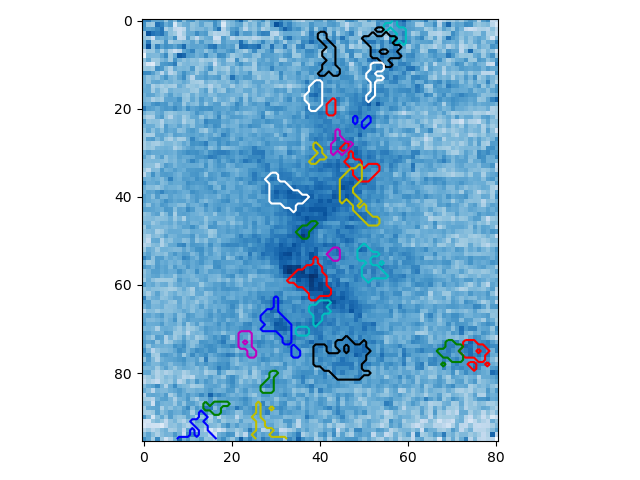
\includegraphics[height=0.45\textheight]{cores.png}
\vspace{-0.5em}
\caption{Contours of the locations of the cores overlayed on an integrated intensity map of the region.}
\vspace{-1em}
\end{figure}

\begin{figure}[H]
\centering
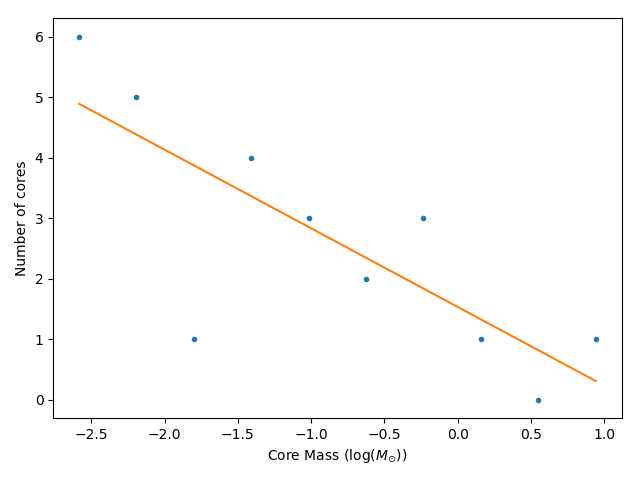
\includegraphics[height=0.45\textheight]{cmf.png}
\vspace{-0.5em}
\caption{The core mass function for the region. Here the fitted line has a slope of $-1.300\pm0.359$.}
\end{figure}
\end{tight_enumerate}



\newpage
\section*{Problem 2. Twinkling Stars: Infrared Luminosity as a Star Formation Rate Tracer}
We use a variety of indirect indicators ot measure the star formation rate in galaxies, and one of the most common is to measure the galaxy's infrared luminosity. The underlying assumptions behind this method are that (1) most of the total radiant output in the galaxy comes from young, recently formed stars, and (2) that in a sufficiently dusty galaxy most of the starlight will be absorbed by dust grains within the galaxy and then re-radiated in the infrared. We will explore how well this conversion works using the popular stellar population synthesis package Starburst99 (Leitherer et al., 1999; V\'azquez \& Leitherer, 2005), \url{http://www.stsci.edu/science/starburst99/}.

\begin{tight_enumerate}
\item Once you have read enough of the papers to figure out what Starburst99 does, use it with the default parameters to compute the total luminosity of a stellar population in which star formation occurs continuously at a fixed rate $\dot{M}$. What is the ratio of $L_{tot}/\dot{M}$ after $10$ Myr? After $100$ Myr? After $1$ Gyr? Compare these ratios to the conversion factor between $L_{TIR}$ and $\dot{M}$ given in Table 1 of Kennicutt \& Evans (2012).

\item Plot $L_{tot}/\dot{M}$ as a function of time for this population. Based on this plot, how old does a stellar population have to be before $L_{TIR}$ becomes a good tracer of the total star formation rate?

\item Try making the IMF slightly top-heavy, by removing all stars below $0.5\ \si{\msun}$. How much does the luminosity change for a fixed star formation rate? What do you infer from this about how sensitive this technique is to assumptions about the form of the IMF?
\end{tight_enumerate}

\subsection*{Solution 2}
\begin{tight_enumerate}
% TODO
\item Without loss of generality, we set the star formation rate to be $\dot{M} = 1$ \si{\msun/yr}. After $10$ \si{\mega{yr}} $\log{L} = 43.326$ \si{ergs\per\second}, so $\left(\frac{L_{tot}}{\dot{M}}\right)|_{t=10\ \si{\mega{yr}}} \sim 43.326$. After $100$ \si{\mega{yr}} $\log{L} = 43.486$ \si{ergs\per\second}, so $\left(\frac{L_{tot}}{\dot{M}}\right)|_{t=100\ \si{\mega{yr}}} \sim 43.486$. After $1$ \si{\giga{yr}} $\log{L} = 43.606$ \si{ergs\per\second}, so $\left(\frac{L_{tot}}{\dot{M}}\right)|_{t=1\ \si{\giga{yr}}} \sim 43.606$. From Kennicutt \& Evans (2012), the conversion factor between $L_{TIR}$ and $\dot{M}$ (SFR) is $43.41$, which lies somewhere between the values at $t = 10$ \si{\mega{yr}} and $100$ \si{\mega{yr}}. 

% TODO
\item $L_{TIR}$ becomes a good tracer of the total star formation rate when this conversion factor matches the exponent given in the ratios. Solving for when these two are equal, we find that the age of a stellar population must be around $28.838$ \si{\mega{yr}} in order for $L_{TIR}$ to be a good tracer. We notice in the graph that there is a "bend" at this point; this is likely a numerical artifact because the maximum mass of the galaxy (following the default values of Starburst99) was set at $10^{6}$ \si{\msun}.

\begin{figure}[h]
\centering
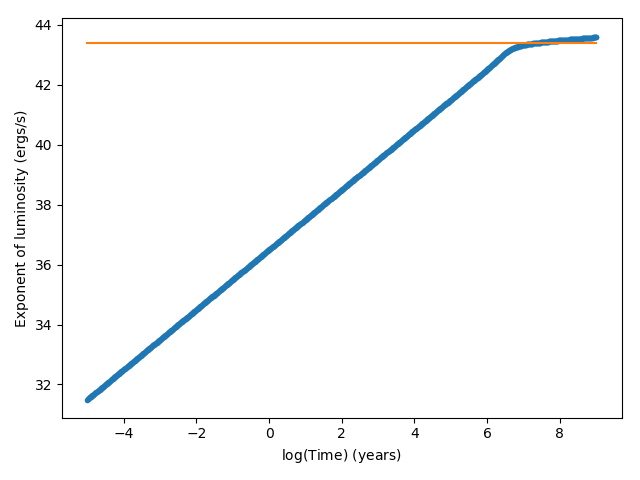
\includegraphics[height=0.45\textheight]{const_lum.png}
\vspace{-0.5em}
\caption{The luminosity of a simulated galaxy given a constant $\dot{M} = 1$ \si{\msun\per{yr}}. Here the orange line indicates the conversion factor between $L_{TIR}$ and $\dot{M}$ from Kennicutt \& Evans (2012).}
\end{figure}

\item For a fixed star formation rate, we find that there is very little difference between our "normal" IMF and this truncated IMF. We find that on average, the exponents of the luminosity vary by $0.3\%$. At $t = 1$ \si{\giga{yr}}, this corresponds to a difference in the luminosity of only $36.46\%$. Given that we have removed a significant fraction of the stellar population, we find that this seemingly small change in luminosity is fairly surprising. Although no such analysis was done for the other case (only low-mass stars), this small discrepancy suggests that this technique is fairly insensitive to the lower masses of the IMF. Since this regime is difficult to observationally constrain, it makes sense that we don't really know the universal IMF behavior at low masses.
\end{tight_enumerate}

\end{document}